\title{Chapter 4, Section 2. Exercises 1, 2, and 4 through 9}
\author{
	MTH 594, Prof. Mikael Vejdemo-Johansson \\
	Differential Geometry Independent Study \\
	\\
	Matthew Connelly \\
}
\date{\today}



\documentclass[12pt]{article}

\usepackage[top=.5in, bottom=.75in, left=1in, right=1in]{geometry}
\usepackage{amssymb}
\usepackage{amsmath}
\usepackage{graphicx}
\usepackage{subcaption}

\newcommand{\ulind}[1]
{
\noindent
\underline{#1}\\\\
\indent
}

\newcommand{\norm}[1]
{
||#1||
}

\newcommand{\oneimg}[2]
{
\begin{figure}[h!]
\centering
\begin{subfigure}[b]{#1\linewidth}
\includegraphics[width=\linewidth]{#2}
\end{subfigure}
\end{figure}
\indent
}

\begin{document}
\maketitle

\section*{Exercise 4.2.6}
\indent
A \emph{helicoid} is the surface swept out by an aeroplane propeller, when both the aeroplane and its propeller move at constant speed. If the aeroplane is flying along the $z$-axis, show that the helicoid can be parametrized as
$$
\sigma(u, v) = (v \cos u, v \sin u, \lambda u)
$$
where $\lambda$ is a constant. Show that the cotangent of the angle that the standard unit normal of $\sigma$ at a point $p$ makes with the $z$-axis is proportional to the distance of $p$ from the $z$-axis.

\vspace{1cm}
\hrule
\vspace{1cm}
\noindent

In $\sigma$, $v$ can be taken to represent the radius of the propeller of the plane (or just the length of a single blade, considering the length of propeller blades should be uniform).\\
\indent
$u$ will then be the angle the propeller is making with some horizontal ($x$-axis) and represent how many rotations the propeller has made in radians cumulatively.\\
\indent
Lastly, $\lambda$ will represent the distance the plane has traveled in the direction of $z$.\\

\begin{figure}[h!]
\centering
\begin{subfigure}[b]{0.4\linewidth}
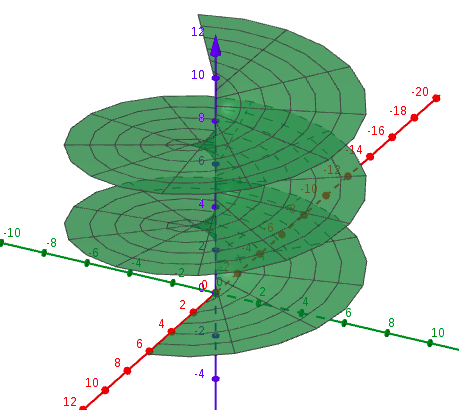
\includegraphics[width=\linewidth]{./assets/4-2-6/helicoid1.png}
\end{subfigure}
\end{figure}
\indent

\ulind{Finding $\sigma$'s unit normal}
$\sigma$'s unit normal can be computed as follows:

$$
\hat{n} = \frac{\sigma_u \times \sigma_v}{||\sigma_u \times \sigma_v||}
$$

But first, its normal is:

$$
\sigma_u \times \sigma_v = n = (-\lambda \sin u, \lambda \cos u, -v)
$$

And the norm of the normal is:

$$
||n|| = \sqrt{\lambda^2 \sin^2 u + \lambda^2 \cos^2 u + v^2}\\
$$
$$
= \sqrt{\lambda^2 + v^2}
$$

$\therefore$, the unit normal to $\sigma$ is:
$$
\hat{n} = \left(\frac{-\lambda \sin u}{\sqrt{\lambda^2+v^2}}, \frac{\lambda \cos u}{\sqrt{\lambda^2+v^2}}, \frac{-v}{\sqrt{\lambda^2+v^2}}\right)
$$

\clearpage

\ulind{Relating the angle that $\hat{n}$ makes with the $z$-axis to its \emph{distance} from the $z$-axis:}

To find the cotangent of the angle that $\hat{n}$ makes with the $z$-axis when $\hat{n}$ is at a point $p$, we'll need $\sin \theta$ and $\cos \theta$. We can find these values by dotting and crossing $\hat{n}$ with the standard unit vector $k = <0,0,1>$:

$$
k \cdot \hat{n} = \norm{k} \ \norm{\hat{n}}\cos \theta
$$
and
$$
\norm{k \times \hat{n}} = \norm{k} \ \norm{\hat{n}}\sin \theta.
$$

With $\norm{k}$ and $\norm{\hat{n}}$ both equal to $1$, we then arrive at the following results: 

$$
k \cdot \hat{n} = \cos \theta = -\frac{v}{\sqrt{\lambda^2+v^2}}
$$
and
$$
\norm{k \times \hat{n}} = \sin \theta  = \frac{\lambda}{\sqrt{\lambda^2+v^2}}.
$$

Compute the cotangent:

$$
\cot \theta = \frac{\cos \theta}{\sin \theta}
$$
$$
 = -\frac{v}{\sqrt{\lambda^2+v^2}} \ \frac{\sqrt{\lambda^2+v^2}}{\lambda}
$$
$$
= -\frac{v}{\lambda}
$$

To relate this value to the distance of $p$ from the $z$-axis, we first need to look at $p$ as a point at, say, $\sigma(x_0,y_0)$:
$$
p = \sigma(x_0,y_0) = (y_0 \cos x_0,y_0 \sin x_0,\lambda x_0)
$$

Because we are only interested in distance from the $z$-\emph{axis}, we can ignore the $k$-component of $\sigma(x_0,y_0)$ and treat it as a planar function:

$$
p = \sigma(x_0,y_0) = (y_0 \cos x_0,y_0 \sin x_0)
$$

Now to find the distance of $p$ to the $z$-axis (or to the origin in the $xy$-plane):

$$
\norm{p} = \sqrt{y_0^2 \cos^2x_0 + y_0^2 \sin^2 x_0}
$$
$$
= \sqrt{y_0^2}
$$
$$
= y_0
$$

\clearpage

We can see that the distance from $p$ to the $z$-axis is equal to $y_0$ in this case. Knowing that $y_0 \in v$ as $\sigma(x_0,y_0) \in \sigma(u,v)$, looking at $\cot \theta$ again:

$$
-\frac{v}{\lambda}
$$

we could restate the above as:

$$
-\frac{y_0}{\lambda}
$$

which shows that the distance of $p$ from the $z$-axis directly affects $\cot \theta \ \forall \ x,y \in u,v$.

\end{document}
